\chapter{Controllo Predittivo (MPC)}
\label{cap:mpc}

\section{Principi del Receding Horizon}
Il Model Predictive Control (MPC) è  controllo avanzato in cui si ottiene  l'azione di controllo ottimale  risolvendo ad ogni istante di campionamento $k$, un problema di ottimizzazione in anello aperto basato sulla previsione del comportamento futuro del sistema. A differenza delle tecniche di controllo in retro azione dello stato(come LQR Cap.\ref{cap:lqr}), in cui la legge di controllo è calcolata esplicitamente offline ovvero a priori, l'MPC invece lavora on-line con un algoritmo che valuta un'intera sequenza ottima di ingressi futuri. Applica così al sistema solo il primo elemento di tale sequenza e all'istante successivo ($k+1$), viene acquisita una nuova misura dello stato e il problema di ottimizzazione viene risolto nuovamente, traslando l'orizzonte temporale in avanti di un passo. Questo meccanismo, noto come \textit{Receding Horizon}, è fondamentale per garantire la chiusura dell'anello di controllo (feedback) e compensare eventuali disturbi che possono essere presenti nel sistema che si osserva.

\subsection{Formulazione del Problema di Ottimizzazione}
Il problema di ottimizzazione dell'MPC nasce dal problema di dovere guidare lo stato del sistema verso l'origine minimizzando un funzionale di costo. Per un sistema a tempo discreto del tipo $x(k+1) = f(x(k), u(k))$, la cifra di merito è definita su un orizzonte di predizione di lunghezza $N$(passi):
\begin{equation}
	J(x(k), u(\cdot)) = \sum_{j=0}^{N-1} l(x(j), u(j)) + V_f(x(N))
\end{equation}
dove $l(x,u)$ rappresenta il costo di stadio (definito positivo e nullo solo nell'origine) e $V_f(x(N))$ rappresenta il costo terminale. 

Il problema di ottimizzazione che il controllore deve risolvere ad ogni istante $k$ è:
\begin{align}
	\min_{u} \quad & J(x(k), u(\cdot)) \label{eq:mpc_cost}\\
	\text{s.t.} \quad & x(0) = x(k) \nonumber \\
	& x(j+1) = f(x(j), u(j)) \nonumber \\
	& x(j) \in \mathcal{X}, \quad u(j) \in \mathcal{U} \nonumber \\
	& x(N) \in \mathbb{X}_f \nonumber 
\end{align}
I vincoli impongono il rispetto della dinamica del sistema, i limiti fisici sugli stati $\mathcal{X}$ e sugli attuatori $\mathcal{U}$ (che si assumono essere insiemi compatti, ovvero chiusi e limitati, e forzano lo stato finale a terminare in un opportuno insieme invariante $\mathbb{X}_f$.
\subsection{Varianti del Vincolo Terminale}
La stabilità, come dimostrato, richiede di forzare lo stato N-esimo in una regione in cui le proprietà della CLF sono valide, ovvero quando viene applicata l'ultima azione di controllo bisogna assicurare di trovarsi inn una posizione in cui essa riesca a riportare il sistema al set-point. Esistono due formulazioni principali per creare il problema di ottimizzazione dell' mpc:

\subsubsection{Vincolo di Uguaglianza $x(N) = 0$}
In questa formulazione alternativa usata principalmente utilizzata per sistemi non lineari e non linearizzabili intorno a un punto di equilibrio dove non si riesce a calcolare una CLF di controllo, il problema di ottimizzazione viene vincolato affinché lo stato raggiunga esattamente l'origine al termine dell'orizzonte predittivo ($x(N)=0$). In questo modo, l'insieme terminale degenera in un punto $\mathbb{X}_f = \{0\}$ e non è necessario calcolare esplicitamente alcuna CLF. Tuttavia, richiedere di annullare l'errore in esattamente $N$ passi restringe drasticamente il dominio di attrazione del controllore, riducendo l'insieme delle condizioni iniziali per cui l'ottimizzazione ammette soluzione quindi diventano di numero minore le soluzione al problema di ottimizazione che l'mpc può trovare.

\subsubsection{Vincolo di Disuguaglianza $x(N) \in \mathbb{X}_f$}
Questo vincolo è quello normalmente usato nei sistemi lineari e linearizzati, l'implementazione mpc che segue infatti impone che lo stato finale entri all'interno di una regione di sicurezza (il Maximal Invariant Set $\mathcal{O}_\infty$). Ciò permette al controllore di avere un bacino di attrazione (o Dominio di Attrazione $\mathbb{X}_N$,\ref{DominioAttr} molto più ampio, dando così la possibilità all' mpc di trovare ad ogni passo k una soluzione al problema di ottimizzazione riportando lo stato nel sistema nella regizione di convergenza del Control-Invariant-Set dove può essere applicata la legge di controllo locale dell'LQR u=-Kx.

\section{Stabilità e teoremi di Lyapunov}

L'architettura del Model Predictive Control, per sua natura, agisce in anello aperto calcolando un'intera sequenza di azioni ottime, ma chiude il ciclo di retroazione (\textit{Feedback di stato}) applicando al sistema esclusivamente il primo elemento della sequenza, seguendo il principio del \textit{Receding Horizon}. 
Come per ogni strategia di controllo, è fondamentale progettare il regolatore in modo da garantire formalmente che il sistema in anello chiuso sia \textbf{asintoticamente stabile}. Per dimostrare questa proprietà, ci si avvale del Teorema di Lyapunov.

\subsection{Teorema di Lyapunov}
Si consideri un sistema non lineare a tempo discreto del tipo $x(k+1) = f(x(k), u(k))$, assunto per semplicità in forma autonoma $x(k+1) = f(x(k))$, con $f(x)$ continua e $\bar{x} = 0$ un punto di equilibrio. Il teorema afferma che, se esiste una funzione continua $V(x)$, definita positiva in $\bar{x}$, tale per cui la sua variazione rispetto alla traiettoria del sistema $\Delta V(x)$ sia semidefinita o definita negativa, ovvero:
\begin{equation}
	\Delta V(x) = V(f(x)) - V(x) \le 0
\end{equation}
allora l'origine $\bar{x} = 0$ è un punto di equilibrio stabile del sistema. Inoltre, se $\Delta V(x) < 0$, l'equilibrio risulta \textbf{asintoticamente stabile}.

\subsection{L'Ipotesi Base di Stabilità nell'MPC}
Senza perdita di generalità, si consideri il problema di regolazione dello stato all'origine ($\bar{x} = 0$). Il problema di ottimizzazione dell'MPC prevede la minimizzazione della seguente cifra di merito:
\begin{equation}
	J(x(k), u(\cdot)) = \sum_{j=0}^{N-1} \ell(x(j), u(j)) + V_f(x(N))
\end{equation}
soggetta ai vincoli sul modello $x(j+1) = f(x(j), u(j))$, e ai vincoli chiusi e limitati (\textit{compatti}) sugli stati $x(j) \in \mathcal{X}$ e sugli ingressi $u(j) \in \mathcal{U}$.
L'idea centrale per la prova di stabilità è dimostrare che il \textbf{costo ottimo} calcolato al tempo $k$, definito come $J^0(x(k))$, rispetti le due proprietà fondamentali per essere una funzione di Lyapunov.

\textbf{1. Definitezza Positiva:}
Questa prima proprietà è garantita \textit{by design} scegliendo un costo di stadio $\ell(x,u)$ e un costo terminale $V_f(x)$ che siano funzioni definite positive (tali che $\ell(0,0) = 0$ e $V_f(0) = 0$). Nel caso specifico si adotteranno forme quadratiche: $\ell(x,u) = \|x\|_Q^2 + \|u\|_R^2$.

\textbf{2. Variazione Definita Negativa:}
Per dimostrare che il costo decresce strettamente nel tempo ($\Delta J(x) = J^0(x^+) - J^0(x(k)) \le 0$), supponiamo che al tempo $k$ l'ottimizzatore abbia trovato la sequenza ottima:
\begin{equation}
	\mathbf{u}^0(x) = \{u^0(0;x), u^0(1;x), \dots, u^0(N-1;x)\}
\end{equation}
che genera la corrispondente sequenza ottima di stati predetti $x^0(j;x)$. Il costo ottimo valutato è quindi $J^0(x(k))$. 
All'istante successivo $k+1$ (dove lo stato attuale diviene $x^+$), il risultato dell'ottimizzazione non è ancora noto. Per ovviare a questo problema, si costruisce una sequenza \textbf{fattibile, ma non ottima} traslando la sequenza precedente di un passo e accodando un'azione di controllo finale definita da una legge locale $v = \kappa_f(x) \in \mathcal{U}$:
\begin{equation}
	\tilde{\mathbf{u}} = \{u^0(1;x), u^0(2;x), \dots, u^0(N-1;x), \kappa_f(x^0(N;x))\}
\end{equation}
Affinché questa sequenza sia effettivamente fattibile per il sistema vincolato, si introduce l'\textbf{Ipotesi base di stabilità}: deve esistere una legge di controllo locale $\kappa_f(x) \in \mathcal{U}$ tale che:
\begin{enumerate}
	\item $\forall x \in \mathbb{X}_f$, allora $f(x, \kappa_f(x)) \in \mathbb{X}_f$, ovvero $\mathbb{X}_f$ deve essere un \textit{Control Invariant Set}.
	\item $V_f(f(x, \kappa_f(x))) - V_f(x) \le -\ell(x, \kappa_f(x))$, ovvero il costo terminale deve agire da Control Lyapunov Function (CLF) locale.
\end{enumerate}

\subsection{La Prova Fondamentale di Stabilità}
Impiegando la sequenza sub-ottima $\tilde{\mathbf{u}}$, è possibile calcolarne il costo associato $J(x^+, \tilde{\mathbf{u}})$. Confrontando la sequenza ottima $\mathbf{u}^0(x)$ all'istante $k$ con la sequenza sub-ottima $\tilde{\mathbf{u}}$ all'istante $k+1$, si evince che esse differiscono esclusivamente per il primo e l'ultimo elemento. 
Sottraendo i due costi, i termini della sommatoria intermedia si elidono perfettamente, restituendo:
\begin{equation}
	J(x^+, \tilde{\mathbf{u}}) - J^0(x(k)) = \ell(x^0(N;x), \kappa_f) + V_f(f(x^0(N;x), \kappa_f)) - \ell(x^0(0;x), u^0(0;x)) - V_f(x^0(N;x))
\end{equation}
Raggruppando i termini, si ottiene:
\begin{equation}
	= -\ell(x^0(0;x), u^0(0;x)) + \underbrace{\ell(x^0(N;x), \kappa_f) + V_f(f(x^0(N;x), \kappa_f)) - V_f(x^0(N;x))}_{\le 0 \text{ (per l'ipotesi base di stabilità)}}
\end{equation}
Poiché $\tilde{\mathbf{u}}$ è una soluzione fattibile ma non ottima, per definizione sappiamo che il costo ottimo al passo $k+1$ sarà minore o uguale a quello sub-ottimo: $J^0(x^+) \le J(x^+, \tilde{\mathbf{u}})$.
Di conseguenza, la variazione del costo ottimo è limitata da:
\begin{equation}
	\Delta J(x) = J^0(x^+) - J^0(x(k)) \le J(x^+, \tilde{\mathbf{u}}) - J^0(x(k)) \le -\ell(x^0(0;x), u^0(0;x))
\end{equation}
Siccome $\ell(\cdot)$ è definita positiva, $-\ell(\cdot)$ è strettamente negativa. Questo conclude la prova: il costo decresce in modo monotòno ad ogni passo di campionamento ($\Delta J(x) \le 0$), agendo formalmente come funzione di Lyapunov e assicurando la totale convergenza asintotica del sistema in anello chiuso (QED). L'analisi per i controllori lineari coinciderà poi con la legge LQR analizzata nel Capitolo \ref{cap:12.5}.

\subsection{Formulazione Alternativa: Vincolo Terminale di Uguaglianza}
In taluni casi può risultare difficile calcolare analiticamente una CLF locale o un \textit{control invariant set} adeguato. Una formulazione alternativa per garantire la stabilità dell'MPC consiste nell'imporre un rigido vincolo terminale di uguaglianza:
\begin{equation}
	x(N) = 0
\end{equation}
In questo scenario non è più necessario determinare una funzione $V_f(x)$, poiché imporre che lo stato terminale sia nullo garantisce intrinsecamente che $V_f(x(N)) = 0$, implicando anche che il \textit{terminal invariant set} sia confinato al solo punto $\mathbb{X}_f = \{0\}$.
Lo sviluppo della prova di stabilità rimane concettualmente identico. Si accoda l'azione nulla $\tilde{\mathbf{u}} = \{u^0(1;x), \dots, u^0(N-1;x), 0\}$, che genera la transizione in equilibrio $f(0,0) = 0$. Il calcolo della differenza tra i costi si riduce quindi a:
\begin{equation}
	J(x^+, \tilde{\mathbf{u}}) - J^0(x(k)) = -\ell(x^0(0;x), u^0(0;x))
\end{equation}
Dimostrando nuovamente la decrescita monotòna e rigorosa del costo ottimo.

\section{Analisi degli insiemi invarianti e stabilità robusta}

Per implementare correttamente un MPC lineare è necessario garantire la stabilità asintotica dell'anello chiuso attraverso una scelta rigorosa degli elementi che compongono il problema di ottimizzazione infatti tale stabilità è garantita rispettando specifici requisiti.

\subsection{Ingredienti Fondamentali per la Stabilità}
Per un sistema lineare o linearizzato intorno a un punto di equilibrio a tempo continuo viene discretizzato a tempo discreto $x(k+1) = Ax(k) + Bu(k)$ e poi soggetto a vincoli deve essere progettato del regolatore deve includere i seguenti cinque ingredienti:
\begin{enumerate}
	\item \textbf{Continuità}: Le funzioni $f(x,u) = Ax+Bu$ e il costo di un passo $l(x,u)$ devono essere continue. Nel caso  di sistemi lineari, questa proprietà è intrinsecamente soddisfatta.
	\item \textbf{Compattezza dei Vincoli}: Gli insiemi $\mathcal{X}$ e $\mathcal{U}$ devono essere compatti (chiusi e limitati) e devono contenere l'origine al loro interno, i vincoli sono espressi in questo modo: $x_{min} \le x \le x_{max}$ e $u_{min} \le u \le u_{max}$.
	\item \textbf{Definitezza Positiva}: Il costo di stadio $l(x,u) = \|x\|_Q^2 + \|u\|_R^2$ e il costo terminale $V_f(x) = \|x\|_P^2$ devono essere definiti positivi ($Q \ge 0, R > 0, P \ge 0$).
	\item \textbf{Esistenza della CLF Locale}: Deve esistere una legge di controllo locale $\kappa_f(x)$ tale per cui il costo terminale soddisfi la disuguaglianza di Lyapunov:
	\begin{equation}
		V_f(f(x, \kappa_f(x))) - V_f(x) \le -l(x, \kappa_f(x))
	\end{equation}
	Nel caso lineare, si sceglie la legge LQR $\kappa_f(x) = -Kx$ e $V_f(x) = x^T P x$, dove $P$ risolve l'equazione di Riccati.
	
	\item \textbf{Invarianza del Vincolo Terminale}: Lo stato finale deve essere forzato in un insieme terminale $\mathbb{X}_f$ che sia un \textit{control invariant set}.
\end{enumerate}

\paragraph{Funzione MATLAB:}
La funzione MATLAB sviluppata per calcolare ed impostare questi requisiti si chiama \texttt{mpc\_ingredients}, la cui implementazione completa è consultabile in Appendice \ref{app:mpc_ingredients}.

\section{Implementazione per Sistemi Lineari: Legame con LQR}
\label{cap:12.5}
Nel caso di sistemi lineari $x(k+1) = Ax(k) + Bu(k)$ con funzione di costo quadratica $l(x,u) = \|x\|_Q^2 + \|u\|_R^2$, gli ingredienti per garantire la stabilità derivano direttamente dalla teoria del Controllo Lineare Quadratico (LQR).

La legge di controllo locale stabilizzante viene scelta come $\kappa_f(x) = -Kx$, dove $K$ è la matrice di guadagno ottima dell'LQR. Di conseguenza, il costo terminale che funge da CLF è dato da:
\begin{equation}
	V_f(x) = \|x\|_P^2 = x^T P x
\end{equation}
La matrice $P$ è la soluzione dell'equazione algebrica di Riccati (DARE). Questa scelta è perfetta poiché misura esattamente il costo "da N a infinito". Inserendo $P$ e $K$ nell'ipotesi base di stabilità si verifica che:
\begin{equation}
	(A-BK)^T P (A-BK) - P = -(Q + K^T R K)
\end{equation}
che rappresenta esattamente l'uguaglianza ricavata dall'equazione di Riccati stazionaria, dimostrando la stabilità.

Per completare la formulazione, l'insieme terminale $\mathbb{X}_f$ viene calcolato iterativamente costruendo il \textit{ Invariant Set Massimo} $\mathcal{O}_\infty$, ovvero il più grande insieme di stati per i quali l'evoluzione governata dal controllore lineare $(A-BK)$ rispetta tutti i vincoli di stato e di ingressi fisici dell' aereo  $X_{max}$ e $U_{max}$.
\subsection{Il Control Invariant Set e il Maximal Invariant Set $\mathcal{O}(\infty)$}
Un \textbf{Control Invariant Set} $\mathbb{X}_f$ è una regione dello spazio degli stati tale per cui, se lo stato vi appartiene allora esiste un comando ammissibile capace di mantenere durante l'evoluzione del sistema all'interno dell'insieme. 
\begin{equation}
	\mathbb{X}_f = \{x \in \mathcal{X} : \text{se } x \in \mathbb{X}_f \implies (Ax + B\kappa_f(x)) \in \mathbb{X}_f, \kappa_f(x) \in \mathcal{U}\}
\end{equation}

Per l'MPC, questo insieme funge da \textit{ancora} per la fattibilità ricorsiva (\textit{recursive feasibility}): garantisce che se il problema è risolvibile al tempo $k$, lo stato terminale $x(N)$ atterrerà in una zona da cui è sempre possibile calcolare una traiettoria futura sicura.

\subsubsection{Algoritmo Iterativo per il Calcolo di $\mathcal{O}(\infty)$}
Per determinare il \textbf{l' Invariant Set} $\mathcal{O}(\infty)$, ovvero il più grande insieme invariante possibile data una legge di controllo LQR $\kappa_f(x) = -Kx$, si utilizza un algoritmo iterativo. 
Si raccolgono i vincoli sullo stato e sugli ingressi in forma matriciale $Gx \le g$:
\begin{equation}
	G = \begin{bmatrix} I \\ -I \\ -K \\ K \end{bmatrix}, \quad g = \begin{bmatrix} X_{max} \\ -X_{min} \\ U_{max} \\ -U_{min} \end{bmatrix}
\end{equation}
Una volta fatto l'algoritmo procede come segue:
\begin{enumerate}
	\item \textbf{Passo 0}: Si definisce $\mathcal{O}(0) = \{x : Gx \le g\}$.
	\item \textbf{Passo $j$}: Si aggiungono i vincoli sullo stato proiettato al passo $j$ tramite la dinamica in loop chiuso $A_{cl} = (A-BK)$:
	\begin{equation}
		\mathcal{O}(j) = \{x \in \mathcal{O}(j-1) : G(A-BK)^j x \le g\}
	\end{equation}
	\item \textbf{Convergenza}: L'algoritmo termina quando $\mathcal{O}(j+1) = \mathcal{O}(j)$, indicando che sono state incluse tutte le limitazioni dinamiche. Il set risultante è l'invariante massimo $\mathcal{O}(\infty)$.
\end{enumerate}
\subsection{Definizione del Punto di Equilibrio e Variabili di Trim}
Prima di procedere con la sintesi del controllore Model Predictive Control (MPC), \`e fondamentale definire il punto di equilibrio (o \textit{Trim Point}) attorno al quale il modello matematico non-lineare dell'F-16 \`e stato linearizzato. Il velivolo in volo livellato non accelerato deve bilanciare perfettamente le forze aerodinamiche (portanza e resistenza) con la spinta del motore e il peso.
Le variabili di trim principali calcolate dall'algoritmo di ottimizzazione sono:
\begin{itemize}
	\item \textbf{$V_{t0}$ (Velocit\`a Totale di Trim)}: La velocit\`a vera a cui il velivolo mantiene il volo livellato.
	\item \textbf{$\theta_{trim}$ (o \texttt{best\_theta})}: L'angolo di beccheggio di equilibrio. In volo livellato, poich\'e l'angolo di rampa $\gamma$ \`e nullo, l'angolo di beccheggio coincide esattamente con l'angolo di attacco $\alpha_{trim}$. Questo valore rappresenta l'inclinazione "a muso in s\`u" necessaria per generare la portanza necessaria a sostenere il peso del velivolo alla velocit\`a $V_{t0}$.
	\item \textbf{$\mathbf{u}_{trim}$ (o \texttt{best\_u})}: Il vettore degli ingressi di equilibrio, composto da:
	\begin{itemize}
		\item Spinta del motore ($T_{trim}$): necessaria per contrastare la resistenza aerodinamica.
		\item Deflessione dell'elevatore ($\delta_{e, trim}$): necessaria per azzerare il momento di beccheggio ($C_m = 0$).
		\item Deflessione dei flaperon ($\delta_{f, trim}$): contribuisce al bilanciamento longitudinale e al profilo di portanza.
	\end{itemize}
\end{itemize}
Poich\'e l'MPC utilizza un modello lineare dinamico tempo-invariante (LTI), il vettore di stato $\mathbf{x}$ e il vettore di ingresso $\mathbf{u}$ del controllore non rappresentano valori assoluti, bens\`i \textbf{perturbazioni} rispetto al punto di trim:
\begin{equation}
	\mathbf{x} = \mathbf{x}_{assoluto} - \mathbf{x}_{trim}, \quad \mathbf{u} = \mathbf{u}_{assoluto} - \mathbf{u}_{trim}
\end{equation}
\subsection{Impostazione dei Vincoli di ingresso e stato}
Il vantaggio principale del controllo predittivo \`e la sua capacit\`a di gestire esplicitamente i vincoli del sistema durante l'ottimizzazione. Nell'applicazione all'F-16, i vincoli sono stati definiti tenendo conto sia dell'inviluppo di volo sicuro sia dei limiti fisici degli attuatori.
\subsubsection{Vincoli di Ampiezza sugli Attuatori}
Gli attuatori meccanici (elevatore e flaperon) e il motore hanno escursioni minime e massime. Per applicare questi vincoli all'ottimizzatore, i limiti assoluti vengono traslati rispetto alla condizione di trim:
\begin{equation}
	\mathbf{u}_{min} - \mathbf{u}_{trim} \le \mathbf{u}(k) \le \mathbf{u}_{max} - \mathbf{u}_{trim}
\end{equation}
Ad esempio, se l'elevatore pu\`o muoversi fisicamente tra $-25^\circ$ e $+25^\circ$, e il valore di trim \`e $+2^\circ$, l'MPC avr\`a a disposizione un'escursione asimmetrica $\delta_e \in [-27^\circ, +23^\circ]$. Questo assicura che il controllore non calcoli mai azioni fisicamente irrealizzabili.
\subsubsection{Vincoli di Rate (Velocit\`a di Attuazione)}
I servomotori reali non possono variare la deflessione istantaneamente. Lo stesso vale per la dinamica della turbina. \`E stato quindi introdotto un vincolo stringente sulla variazione dell'ingresso tra un istante di campionamento e il successivo:
\begin{equation}
	-\Delta\mathbf{u}_{max} \le \mathbf{u}(k) - \mathbf{u}(k-1) \le \Delta\mathbf{u}_{max}
\end{equation}
Questo vincolo \`e essenziale non solo per il realismo ingegneristico, ma previene anche il chattering (oscillazioni ad alta frequenza) nel segnale di controllo, prolungando la vita utile degli attuatori.
\subsubsection{Vincoli sugli Stati}
I vincoli sugli stati impediscono al velivolo di entrare in regimi aerodinamici pericolosi. Nello specifico, si \`e limitata l'escursione dell'angolo di beccheggio $\theta$ e della velocit\`a angolare $q$ per evitare il superamento dell'angolo di stallo e per mantenere le ipotesi di linearit\`a del modello attorno al punto di equilibrio. Anche in questo caso, i bounds vengono centrati sullo stato di trim:
\begin{equation}
	\mathbf{x}_{min} \le \mathbf{x}(k) \le \mathbf{x}_{max}
\end{equation}

\subsection{Definizioni di Insiemi Controllabili e Stabilizzabili}
\label{DominioAttrazione}
Per definire gli insiemi controllabili e stabilizzanti serve una caratteristica molto importante ovvero il  \textbf{Dominio di Attrazione} $\mathbb{X}_N$, ovvero, (l'insieme di tutti gli stati iniziali da cui lo stato iniziale di un sistema può essere controllato in $N$ passi e riportato all'orgine o a un set-point diverso dall' origine), è necessario quindi definire la gerarchia degli insiemi:

\subsubsection{One-step Set $\mathcal{Q}(\Omega)$}
Questo insieme rappresenta l'insieme degli stati $x \in \mathcal{X}$ per i quali esiste almeno un comando ammissibile $u \in \mathcal{U}$ capace di portare il sistema nel set target $\Omega$ in un solo passo:
\begin{equation}
	\mathcal{Q}(\Omega) = \{x \in \mathcal{X} : \exists u \in \mathcal{U} \text{ s.t. } (Ax+Bu) \in \Omega\}
\end{equation}

\subsubsection{i-steps Controllable Set $\mathcal{C}_i(\mathcal{X}, \Omega)$}
Questo insieme mostra gli stati che possono essere portati in $\Omega$ in esattamente $i$ passi, rispettando i vincoli di stato lungo tutta la traiettoria:
\begin{equation}
	\mathcal{C}_{i+1}(\mathcal{X}, \Omega) = \mathcal{Q}(\mathcal{C}_i(\mathcal{X}, \Omega)) \cap \mathcal{X}, \quad \text{con } \mathcal{C}_0 = \Omega
\end{equation}

\subsubsection{i-steps Stabilizable Set $\mathcal{S}_i(\mathcal{X}, \Omega)$}
Un insieme si dice \textit{stabilizzabile} in $i$ passi se il target $\Omega$ è un \textbf{invariant set}. 

\subsection{Proprietà di Monotonicità e Convergenza}
Esiste una differenza cruciale tra $\mathcal{C}_i$ e $\mathcal{S}_i$ che determina il successo dell'MPC:
\begin{itemize}
	\item \textbf{Monotonicità di $\mathcal{S}_i$}: Poiché $\Omega$ è invariante, vale sempre la proprietà di inclusione:
	\begin{equation}
		\mathcal{S}_i(\mathcal{X}, \Omega) \subseteq \mathcal{S}_{i+1}(\mathcal{X}, \Omega)
	\end{equation}
	La proprietà mostra che all'aumentare dell'orizzonte di predizione $N$ il dominio di attrazione $\mathbb{X}_N$ non può restringersi. Se uno stato raggiunge il set di sicurezza in $i$ passi, l'invarianza garantisce che possa rimanerci anche al passo $i+1$. Questa inclusione non è garantita per i set controllabili  generici che non hanno un target invariante.
	\item \textbf{Convergenza}: Entrambe le sequenze $\mathcal{S}_i$ e $\mathcal{C}_i$, per $i \to \infty$, convergono allo stesso insieme limite: il \textbf{Maximal Control Invariant Set} $\mathcal{O}_\infty(\mathcal{X})$, che rappresenta la regione massima di governabilità del sistema.
\end{itemize}

L'implementazione dell'MPC utilizza queste proprietà per espandere il dominio di attrazione $\mathbb{X}_N$ rispetto al semplice set invariante locale $\mathbb{X}_f$. Più lungo è l'orizzonte $N$, maggiore è la capacità del controllore di recuperare l'aereo da perturbazioni severe, portandolo gradualmente all'interno della regione di sicurezza $\mathcal{O}_\infty(\mathcal{X})$.

\begin{figure}[!h]
	\centering
	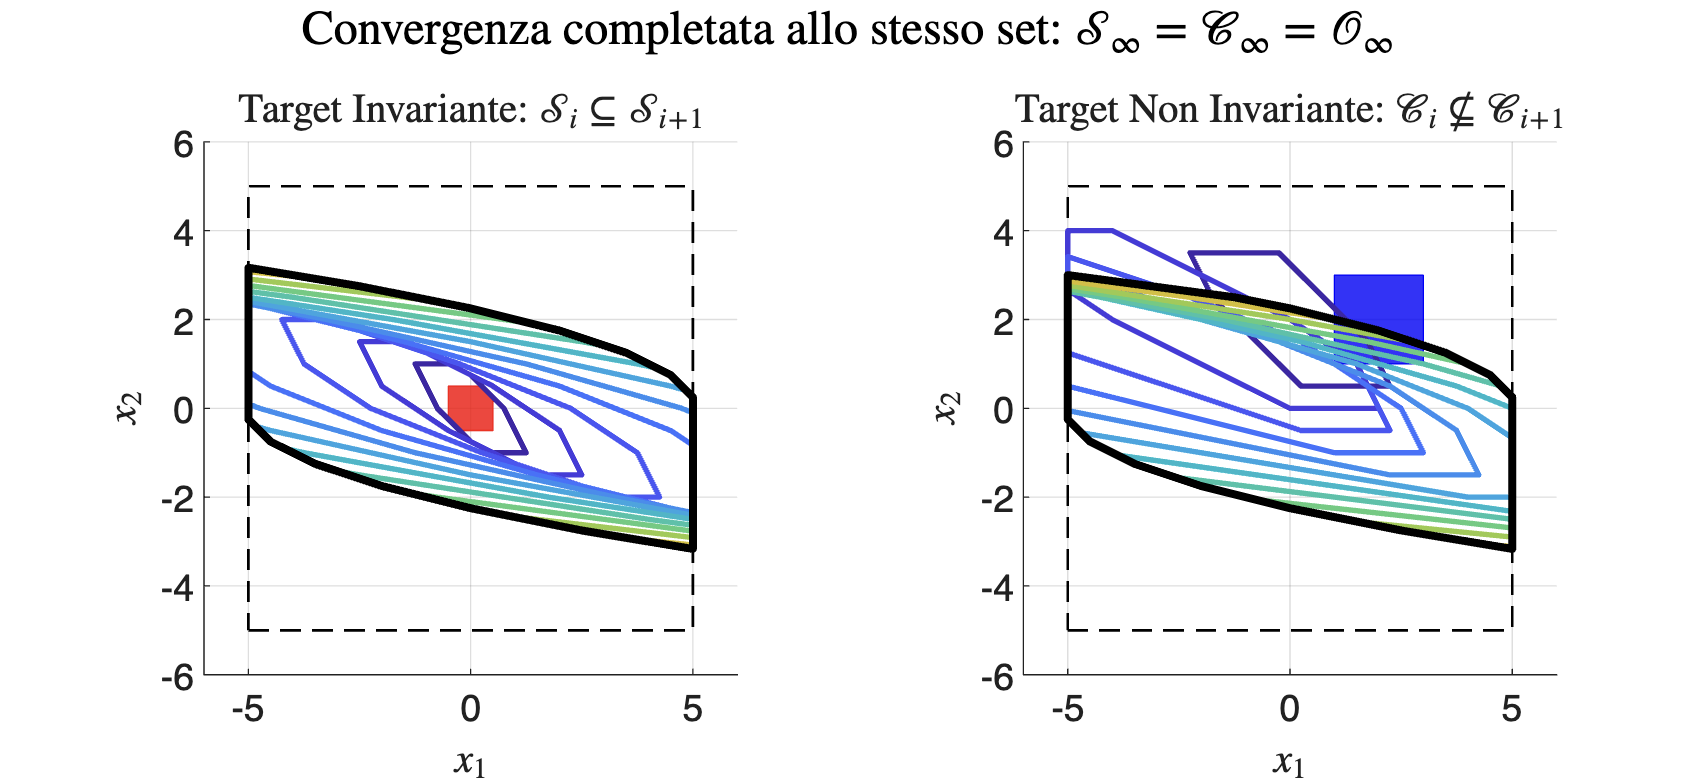
\includegraphics[width=0.85\textwidth]{Foto/mpc/mpc_control_invariant.png}
	\caption{Evoluzione spaziale degli insiemi a $i$ passi. Il grafico confronta visivamente le proprietà matematiche discusse mostrando un target invariante (insiemi stabilizzabili $\mathcal{S}_i$) si ottiene una sequenza in rigorosa espansione monotona, mentre l'utilizzo di un target generico non invariante (insiemi controllabili $\mathcal{C}_i$) non garantisce la proprietà che garantisce la completa controllabilità del sistema in N passi}
	\label{fig:control_set_diff}
\end{figure}
\section{Implementazione Pratica: Controllo Longitudinale F-16}
Alla luce della teoria esposta precedentemente, si è  implementato in MATLAB un controllore MPC per la dinamica longitudinale del velivolo F-16. Il vettore di stato è stato definito secondo l'ordine $[\theta, q, u, w]$, al fine di modellare l'assetto di beccheggio, il pitch rate e le componenti di velocità nel sistema di riferimento \textit{body} del velivolo. 
A causa delle variabili di stato con grandezze fisiche diverse (ad esempio, le velocità $u$ e $w$ misurate in piedi al secondo contro angoli misurati in radianti), le matrici di costo $Q$ ed $R$ sono state penalizzate secondo la teoria di Bryson\cite{Astrom2008}, normalizzando gli errori massimi tollerabili per garantire la corretta penalizzazione delle matrici Q ed R dell'ottimizzatore \texttt{quadprog}.



\subsection{Analisi dei Risultati e Validazione del Controllore MPC}

L'implementazione del controllo predittivo basato su modello (MPC) ha permesso di gestire la dinamica longitudinale del velivolo F-16 garantendo il rispetto rigoroso dei vincoli fisici sugli attuatori e sugli stati, superando i limiti intrinseci del controllo LQR. 

La simulazione è stata condotta a partire da una condizione iniziale molto perturbata, definita nel vettore di stato iniziale $\mathbf{x}_0$ come:
\begin{equation}
	\mathbf{x}_0 = [\theta, q, u, w]^T = [25^\circ, 3^\circ/s, 2\,ft/s, 5\,ft/s]^T
\end{equation}

Nonostante il setpoint iniziale l'algoritmo di ottimizzazione \texttt{quadprog} riesce ad identificare una sequenza di controllo ammissibile all'interno dell'orizzonte predittivo $N=30$ (corrispondente a 1.5 secondi con $T_s = 0.05\,s$).
\label{DominioAttr}
\begin{figure}[!h]
	\centering
	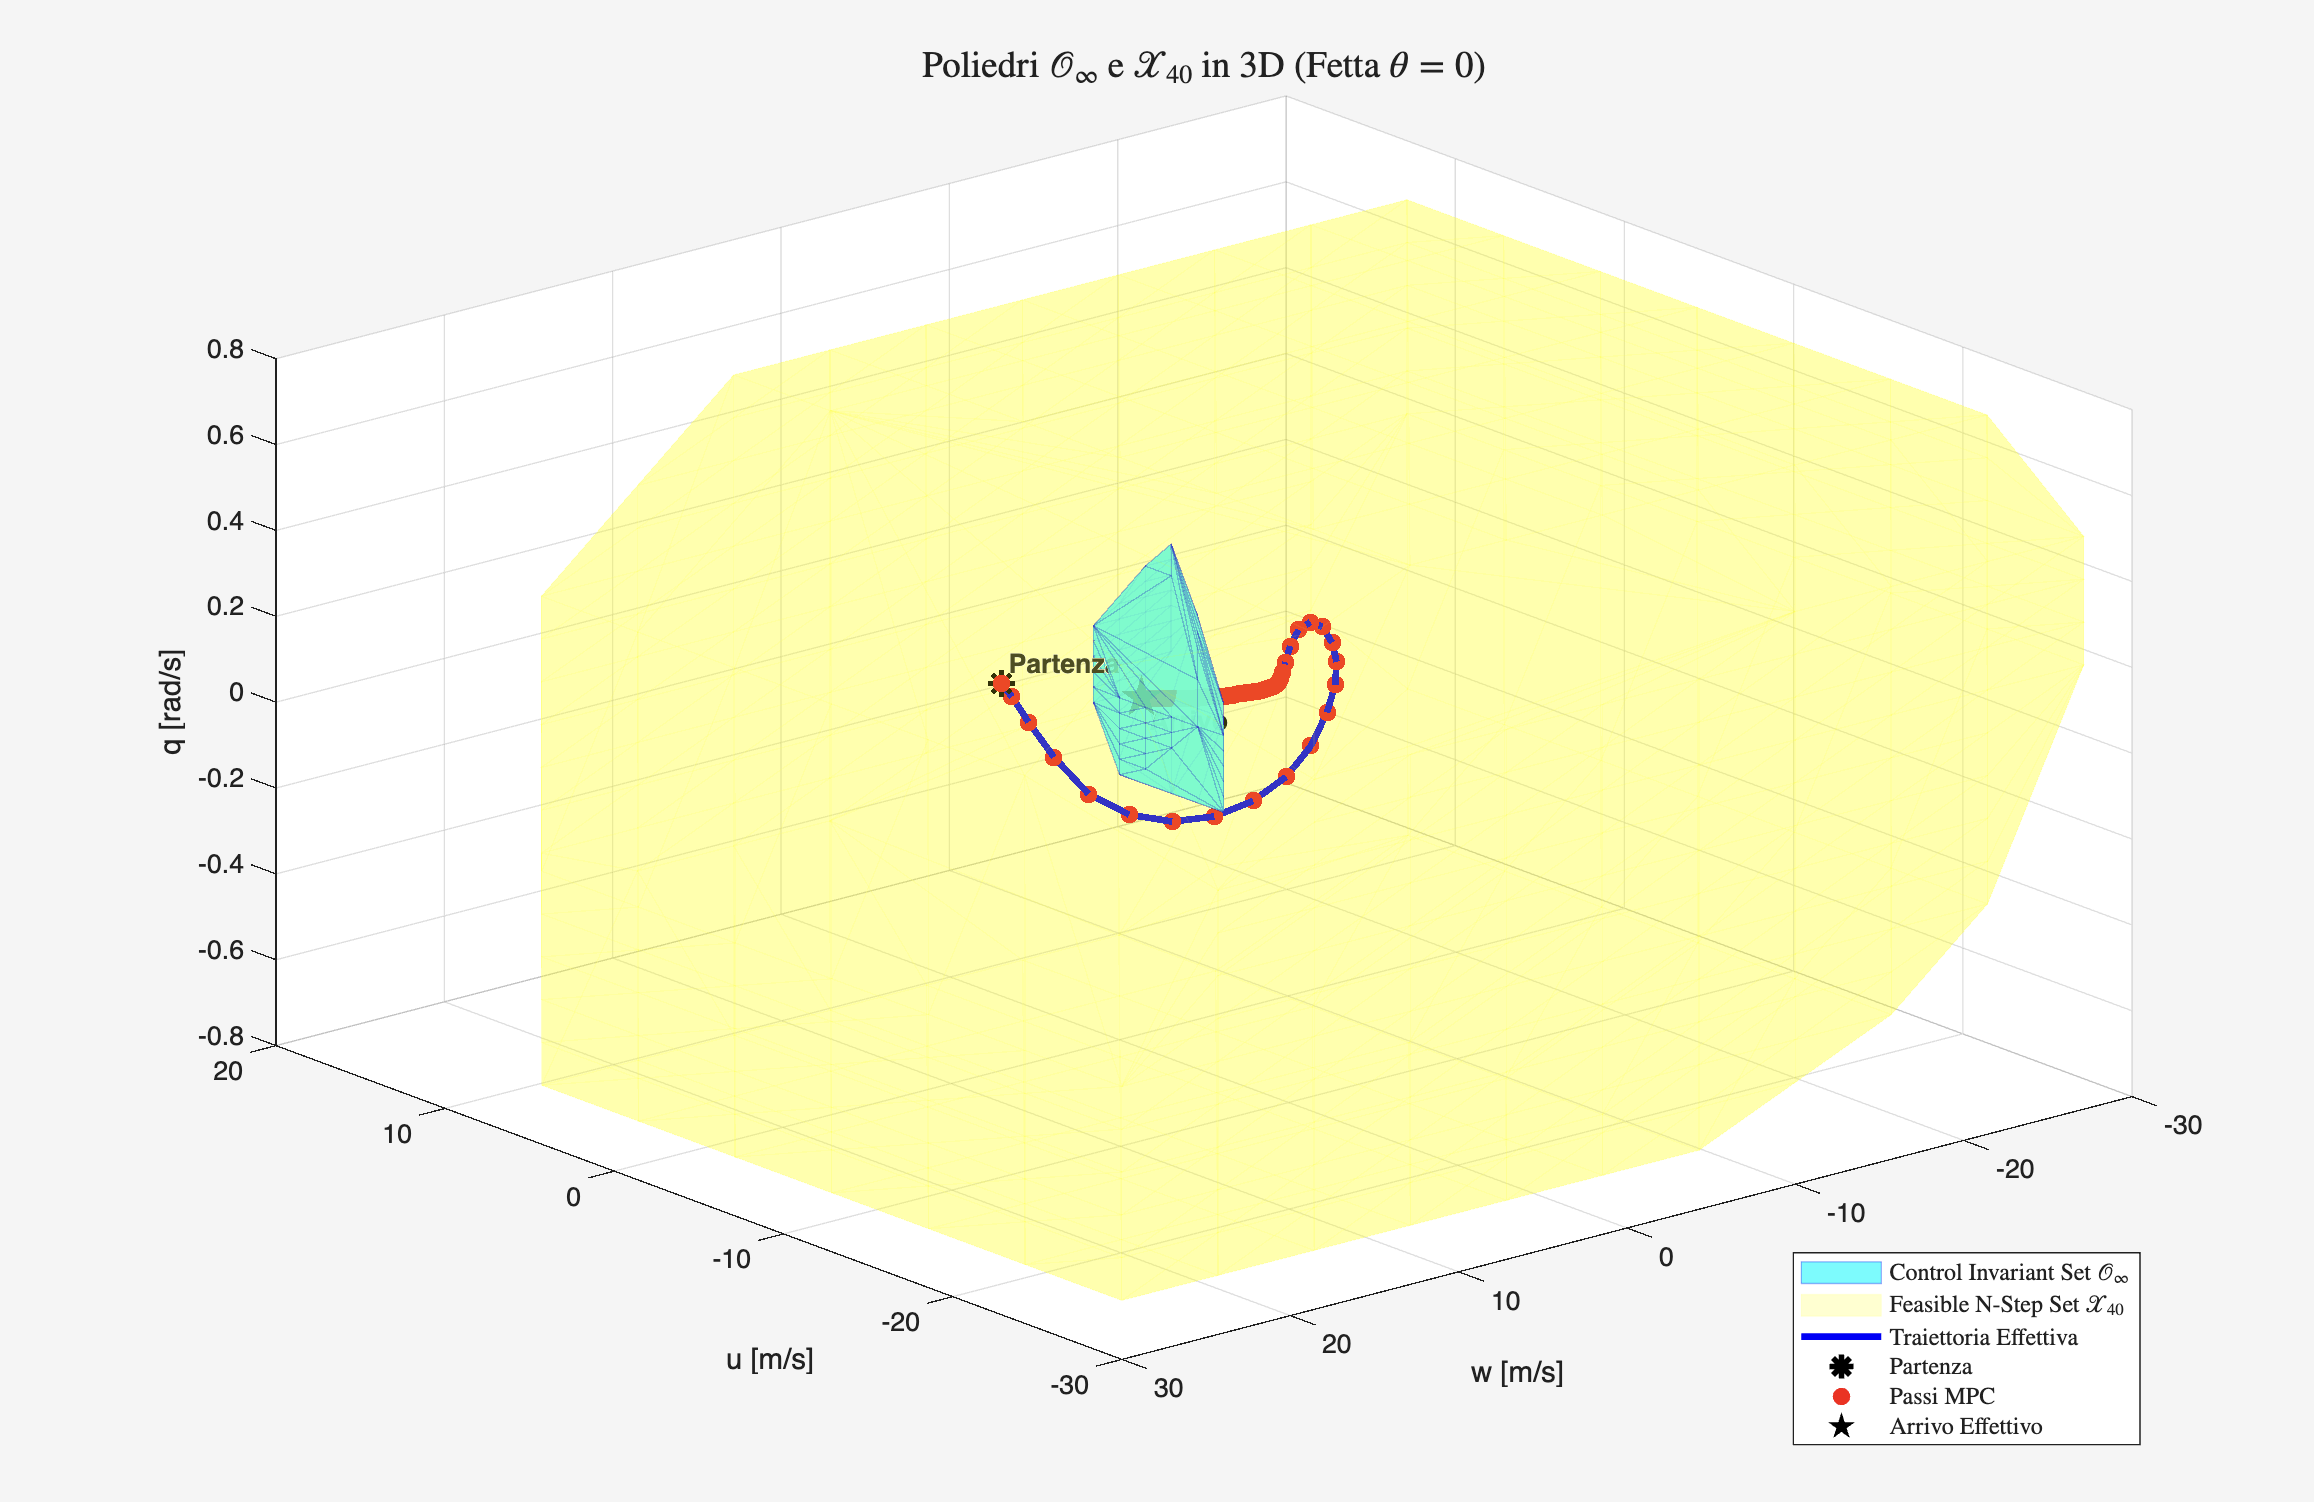
\includegraphics[width=0.7\textwidth]{Foto/mpc/ControlInvariantSet.png}
	\caption{Rappresentazione del poliedro di invarianza $\mathcal{X}_f$ (fetta $\theta=0$) e traiettoria di predizione dello stato verso l'origine.}
	\label{Control-Invariant_set}
\end{figure}

Come evidenziato nella Figura \ref{Control-Invariant_set}, la solidità matematica del controllore è garantita dal calcolo dell'insieme invariante massimale $O_\infty$. Lo script MATLAB ha verificato la convergenza del poliedro, definendo la regione dello spazio di stato entro la quale il sistema può essere stabilizzato senza violare i vincoli. La traiettoria di predizione (visualizzata in rosso) mostra come l'MPC pianifichi come riportare lo stato del sistema verso l'origine forzando lo stato finale a cadere all'interno del \textit{terminal set}, inoltre si mostra la nuvola gialla di possibili stati del sistema che mostra il dominio di attrazione dell' MPC impostato in questa simulazione con N=40, essa mostra l'argomento trattato nella sezione \ref{DominioAttrazione}.

\begin{figure}[!h]
	\centering
	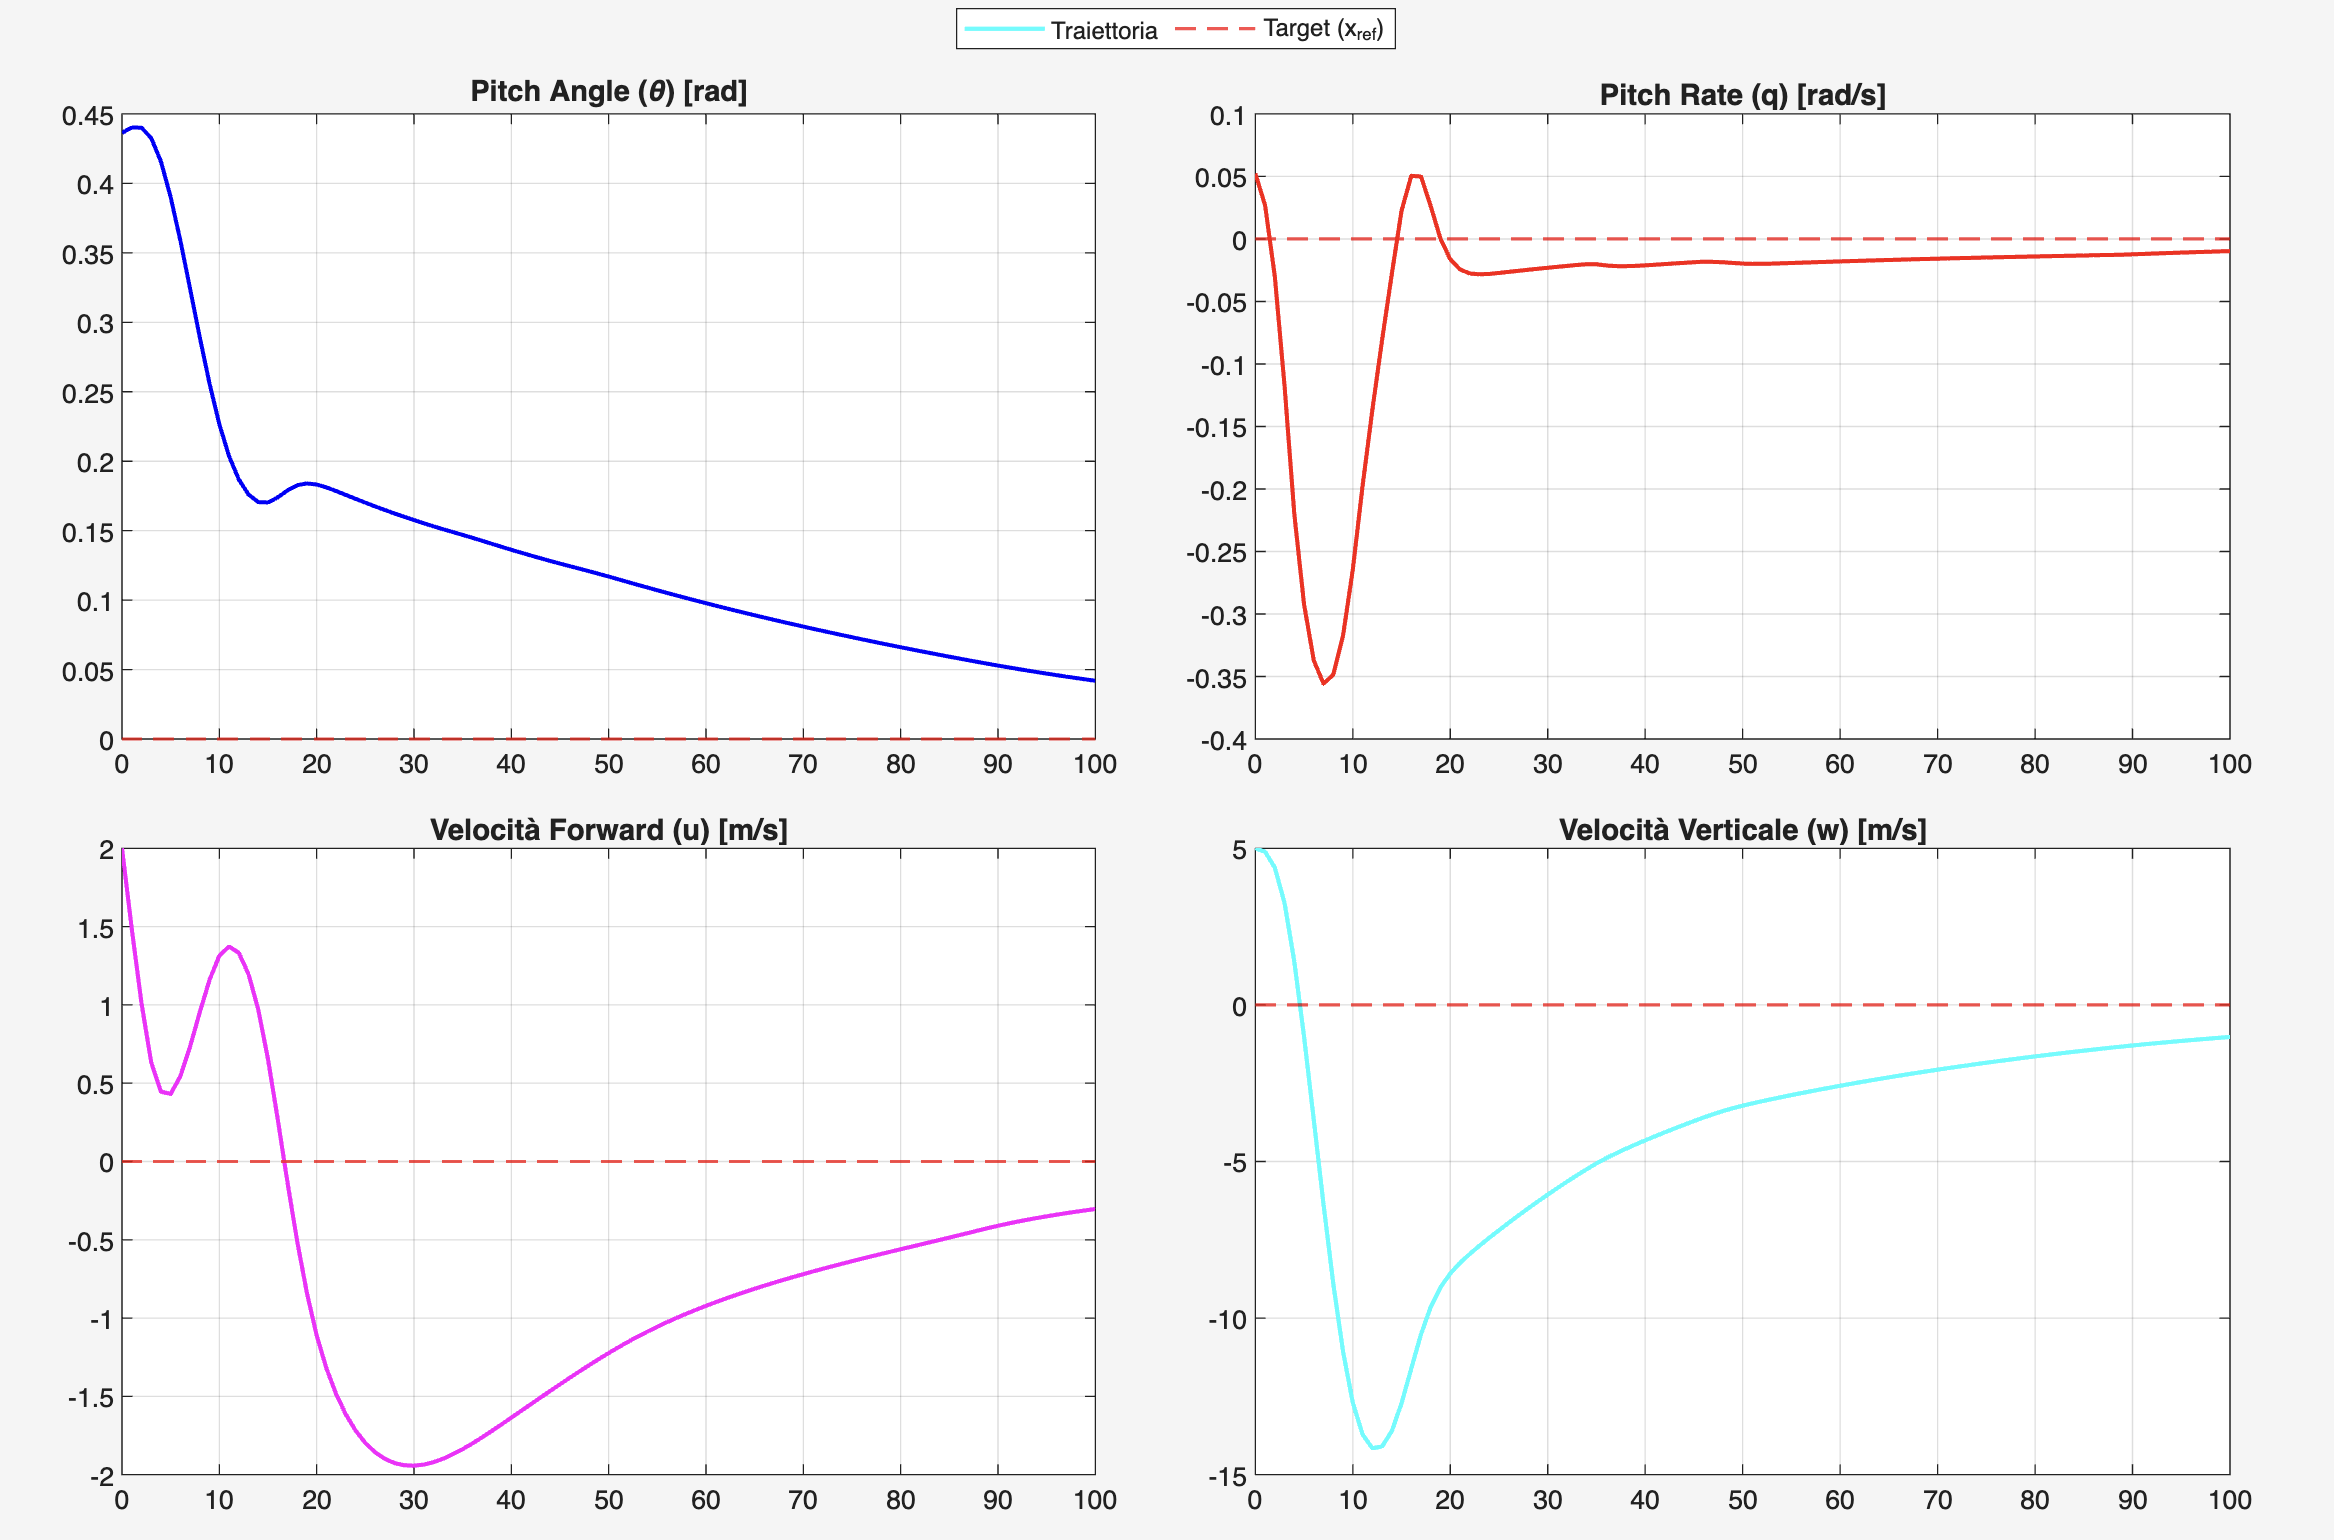
\includegraphics[width=0.7\textwidth]{Foto/mpc/mpcVStato.png}
	\caption{Evoluzione temporale delle variabili di stato: beccheggio, pitch rate e variazioni di velocità lineare.}
	\label{variabili di stato}
\end{figure}

L'analisi degli stati al passare del tempo (Figura \ref{variabili di stato}) mostra un transitorio fluido e privo di sovra-elongazioni critiche per l'angolo di beccheggio e le velocità lineari. Il tempo di assestamento complessivo è coerente con la penalizzazione applicata tramite la matrice $Q$ (calcolata secondo la regola di Bryson)\cite{Astrom2008}, bilanciando correttamente la rapidità di risposta con la stabilità del velivolo. L'aspetto più significativo emerge dalla Figura \ref{ingressi al sistema}, relativa allo sforzo di controllo. A differenza di un regolatore lineare standard, l'MPC sfrutta l'intera autorità di comando disponibile "appoggiandosi" ai vincoli di saturazione ($\pm 25^\circ$ per l'elevatore e $\pm 12^\circ$ per i flap) senza mai superarli. La gestione dei vincoli di rateo (\textit{Rate Limiting}), integrata nella matrice delle disuguaglianze del problema QP, previene variazioni impulsive di spinta, proteggendo l'integrità strutturale dei servomeccanismi dell' aereo, Inoltre, avendo tarato le matrici $Q$ ed $R$ attraverso la regola di Bryson, la matrice $P$ ottenuta dall'equazione di Riccati, su cui si basa la CLF all'interno del control-invariant set, genera un'azione di controllo realistica. Ciò permette al velivolo di compiere manovre rispettando rigorosamente i limiti fisici, pur sacrificando una convergenza più rapida verso l'equilibrio. 

\begin{figure}[!h]
	\centering
	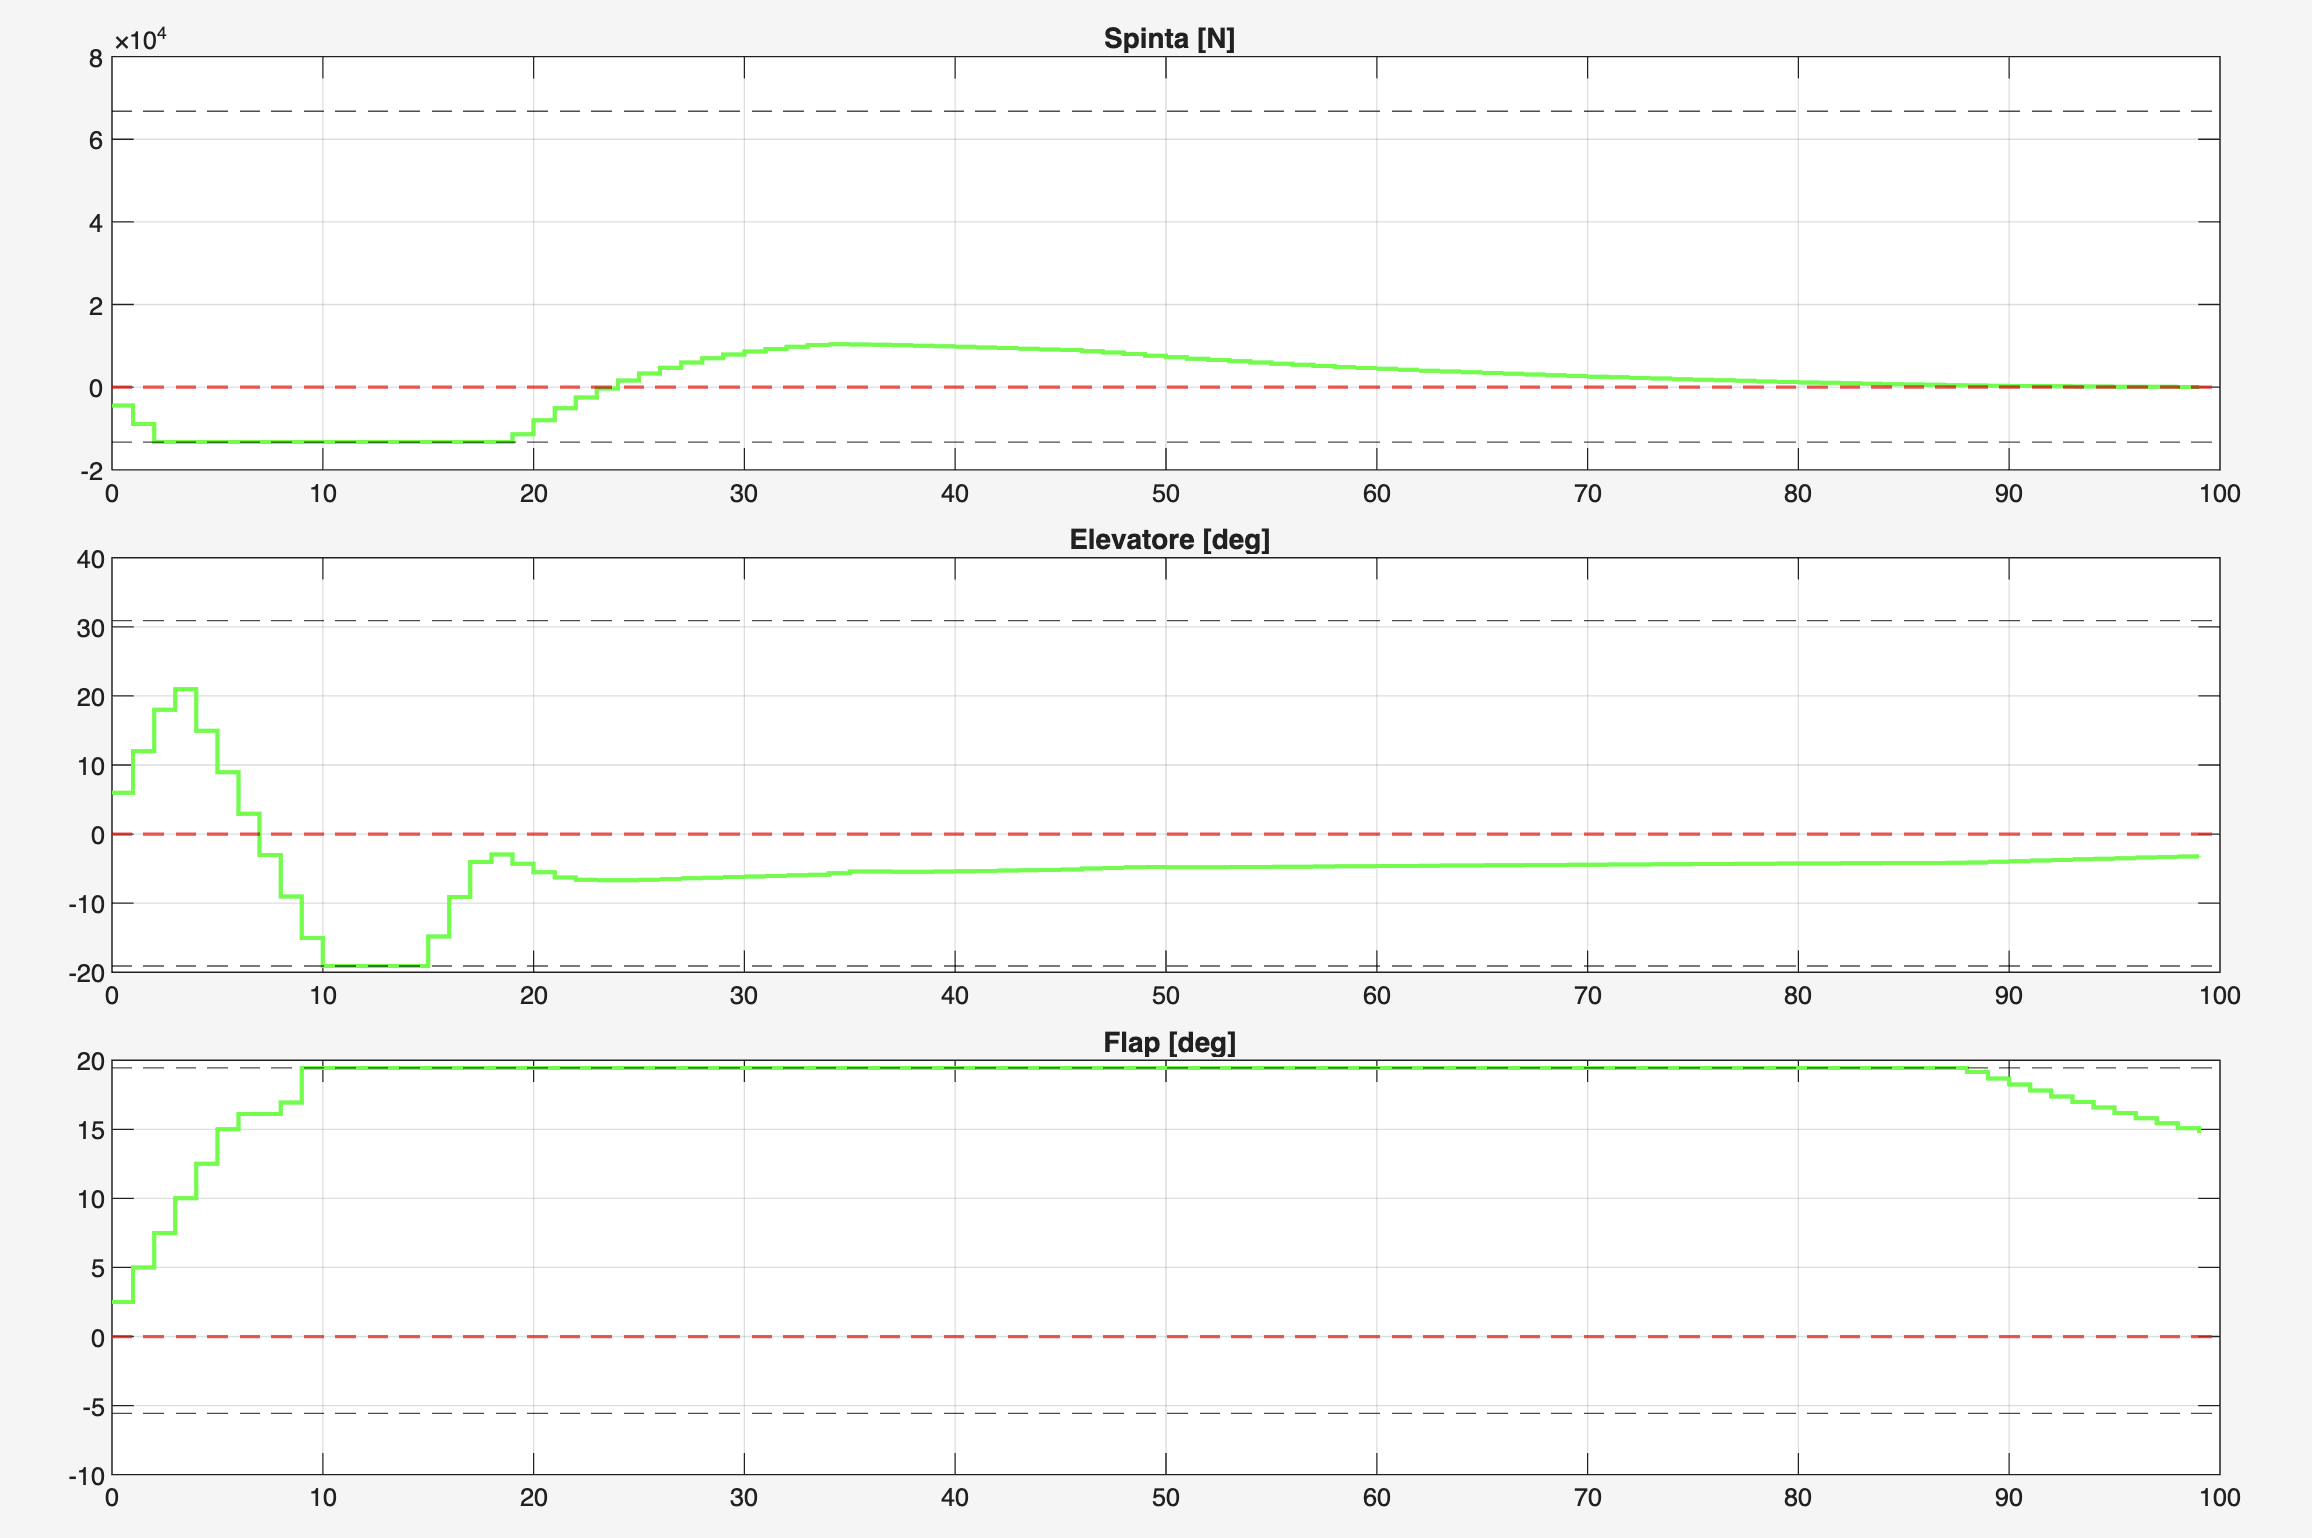
\includegraphics[width=0.7\textwidth]{Foto/mpc/mpcAttuatori.png}
	\caption{Sforzo di controllo degli attuatori: si noti l'attivazione dei vincoli di saturazione sull'elevatore e sui flap.}
	\label{ingressi al sistema}
\end{figure}



% NUOVA SEZIONE: ANALISI GEOMETRICA MPC 
\subsection{Variazione del Funzionale di Costo}

Per completare la validazione del controllore predittivo ed effettuare un confronto diretto con le prestazioni del regolatore LQR analizzate in precedenza, è stata valutata la topologia dello spazio degli stati sottoponendo il sistema al medesimo set di condizioni iniziali multiple $\mathbf{X}_{0,\text{mult}}$. Osservando il comportamento del sistema (Figura \ref{fig:mpc_geometrica}), si nota in modo evidente come il funzionale di costo ottimo calcolato ad ogni passo dal controllore MPC assuma il ruolo di una \textbf{funzione di Lyapunov} per il sistema. Dal grafico tridimensionale emerge chiaramente che, a partire da ogni condizione iniziale, il costo scende monotonamente lungo la superficie definita dalla funzione di costo terminale $V(x) = x^T P x$ (dove $P$ è la matrice di costo finale associata al controllore LQR non vincolato).

\begin{figure}[!h]
	\centering
	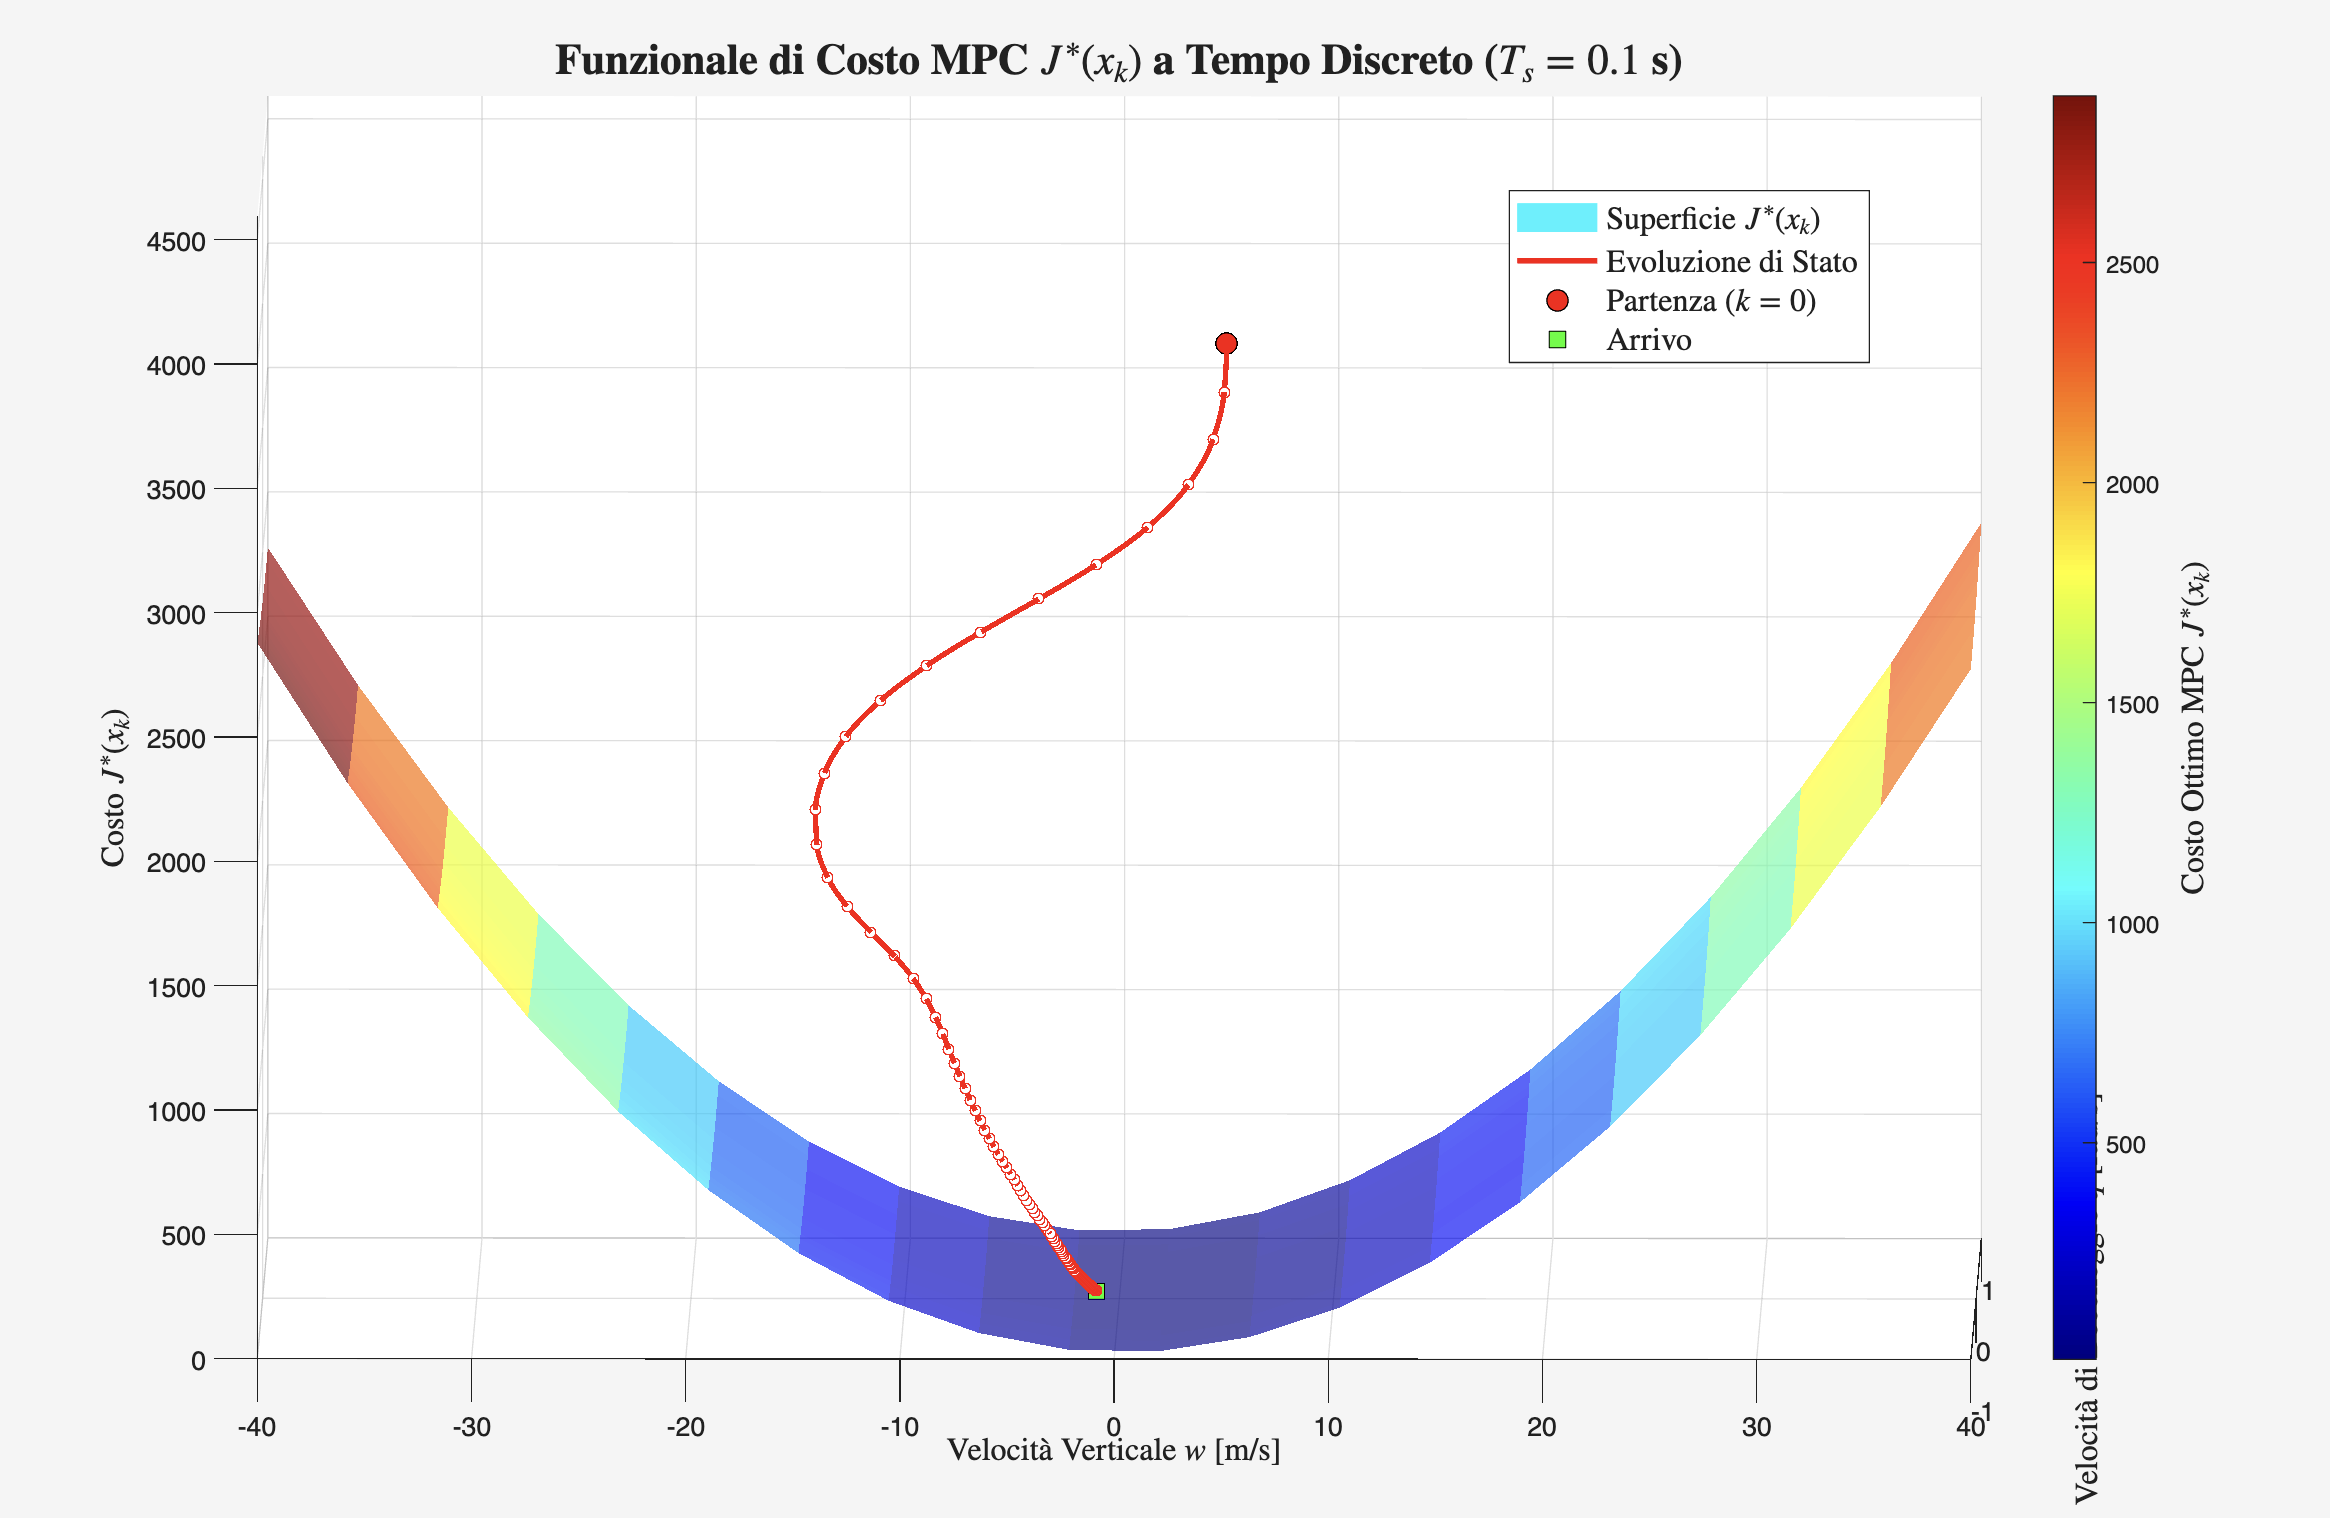
\includegraphics[width=\textwidth]{Foto/mpc/mpc_ljapunov.png}
	\caption{Analisi geometrica del controllore MPC a ciclo chiuso. Il grafico tridimensionale mostra l'evoluzione dello stato e il corrispondente andamento decrescente del funzionale di costo ottimo, che si comporta come una funzione di Lyapunov scendendo lungo la superficie del costo terminale.}
	\label{fig:mpc_geometrica}
\end{figure}



Questo andamento strettamente decrescente nel tempo è la prova geometrica che garantisce la \textbf{stabilità asintotica in anello chiuso}. Infatti, come prescritto dal Teorema di Lyapunov, la variazione negativa del funzionale ad ogni passo ($\Delta J^0(x) < 0$) assicura che le traiettorie siano "attratte" in modo inesorabile verso l'origine, senza la possibilità di divergere o di creare cicli instabili. La stabilità è permessa dalla corretta definizione del tempo di campionamento e del dominio di attrazione dell'MPC, unita alla capacità del \textit{solver} numerico di trovare una soluzione ottima fattibile tra un istante discreto e il successivo. Inoltre, emerge in modo palese la natura ibrida dell'ottimizzazione MPC: man mano che le traiettorie convergono verso l'origine e lo stato rientra all'interno del \textit{Control Invariant Set}, i vincoli smettono di essere attivi (ovvero il sistema non satura più gli attuatori). In quest'area la soluzione dell'MPC converge a quella del regolatore lineare, affidandosi alla legge di controllo ottima locale $u = -Kx$ (identica a quella discussa per il controllore LQR) per guidare definitivamente l'aereo al punto di equilibrio desiderato. In conclusione, i risultati dimostrano che l'architettura MPC è in grado di trasformare un impianto multivariabile fortemente accoppiato in un sistema governabile e robusto. Il controllore garantisce di operare in sicurezza anche in presenza di forti perturbazioni iniziali, assicurando contemporaneamente il rigoroso rispetto dei vincoli fisici e l'assoluta stabilità asintotica del volo.
\part{Implementazione Real-Time Multithreading in C++}
